\section{Data}\label{sec:data}

There are several sources of liquidity in a banking system, those that are not
under  the control  of  a  central bank  and  therefore  represent sources  of
uncertainty. These  are known as \textit{autonomous  factors}.  The autonomous
factors  for   which  forecasting   models  are  built   in  this   study  are
\textit{currency  in  circulation},  the \textit{state  account  balance}  and
\textit{net foreign assets}.  Our data were  obtained from the Central Bank of
the United Arab Emirates (UAE) and are  collected at a daily frequency. We now
discuss each of the autonomous factors in turn.

\subsection{Currency in Circulation}

Currency in  Circulation (CIC)  is the  quantity of  money issued  by monetary
authorities net of currency that has been removed from the money supply.

\textit{\color{blue}  RF to  potentially expand  on CIC  data, how  collected,
measured etc.}

Currency in Circulation  tends to be influenced by calendar  effects.  In many
countries, salaries are paid at the same  time each week (or month) leading to
a smooth weekly (or monthly pattern)  whereby CIC increases after the pay date
and slowly declines until just before the next pay date. The weekly pattern in
CIC  can also  be influenced  by a  tendency of  individuals to  withdraw cash
before the  weekend. Public  holidays can have  a major impact  on CIC,  it is
typical  for CIC  to increase  in the  buildup to  a public  holiday and  then
decline  afterwards. These  systematic features  make it  possible to  develop
models for forecasting CIC at horizons of 1 to 14 days that outperform na\"ive
forecasting techniques.

Figure~\ref{fig:cicdata} highlights  CIC data for  the UAE. Days  with missing
data include  weekends (Friday and  Saturday in  the UAE) and  major holidays.
Data on these  days are linearly interpolated. Other  autonomous factors which
may  exhibit a  different pattern  of missingness  (for instance  data may  be
available on  Fridays for  net foreign assets  since foreign  exchange markets
trade  on  Friday),   are  interpolated  in  a  similar   fashion.   As  such,
interpolating rather than ignoring missing data guarantees a balanced panel of
data, which  becomes important for  reconciliation steps later on.   The daily
pattern  of  CIC is  apparent  from  the figure  as  are  spikes around  major
holidays, in particular Eid al Fitr and Eid  al Adha. In early 2020 there is a
permanent level shift in CIC associated with measures at the onset of Covid to
inject cash into the monetary system.

\begin{figure}[!h] \centering 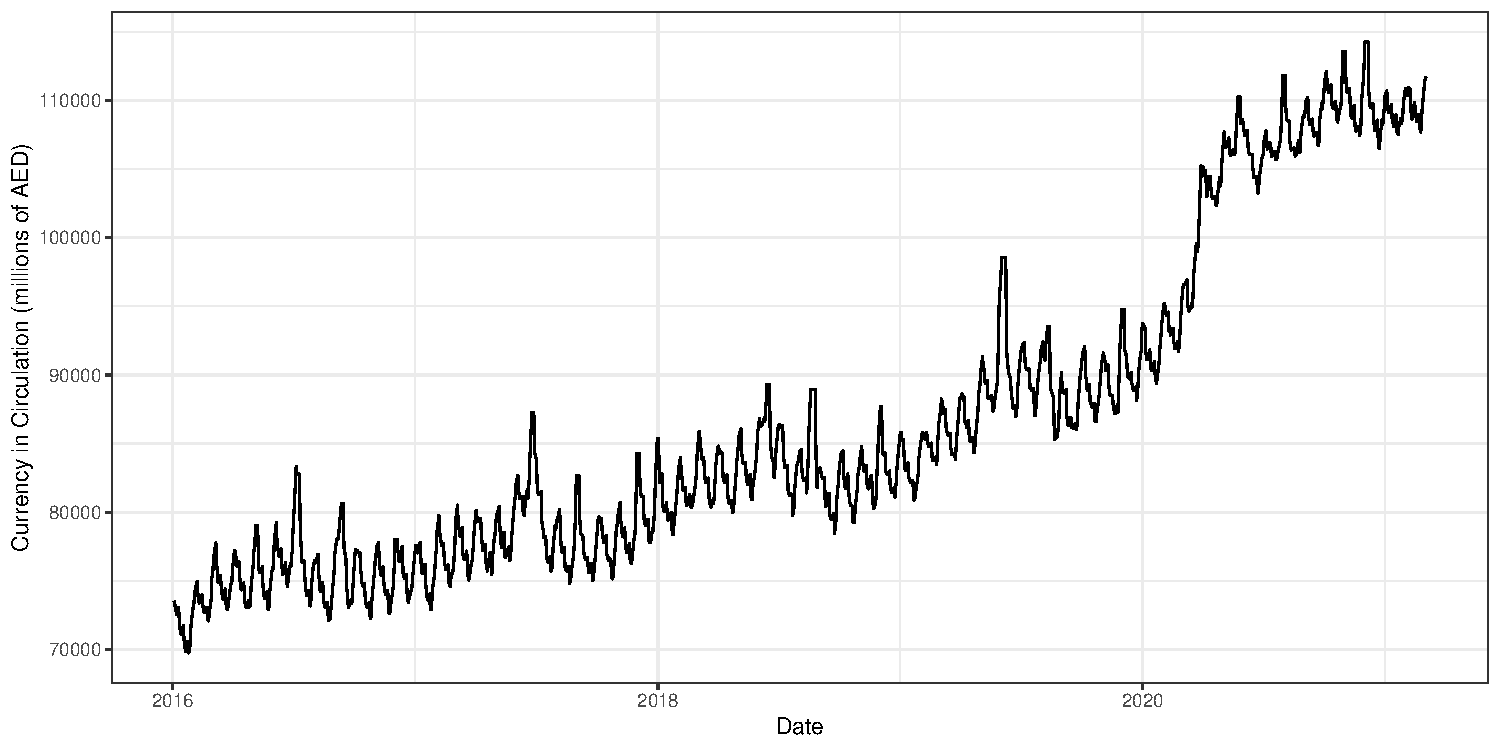
\includegraphics[scale=0.6]{cicplot}
    \caption{Currency  in  Circulation  data  for  the  United  Arab  Emirates
measured in million of Dirhams.}
    \label{fig:cicdata}
\end{figure}

\subsection{State Account Balance}

State Account Balance (SAB) is the quantity of money held by the government in
its account with the Central Bank.

\textit{\color{blue}  RF to  potentially expand  on SAB  data, how  collected,
measured etc.}

State Account  Balance also  tends to  be influenced  by calendar  effects. In
particular certain  taxes may  be due  for collection towards  the end  of the
week, month,  quarter of financial  year which can provide  a boost to  SAB at
these time. Models  accounting for these features can  also outperform na\"ive
approaches in forecasting SAB.

Figure~\ref{fig:sabdata} highlights  SAB data for  the UAE. Apart  from spikes
associated with seasonal factors, there is also a large one off spike in early
2019 associate  with the sale  of government  assets.  In our  modelling, such
transitory effects can  be accounted for via the use  of dummy variables. When
asset  sales are  scheduled to  occur at  some time  in the  future, this  may
motivate judgemental adjustments to model forecasts.

\begin{figure}[!h] \centering 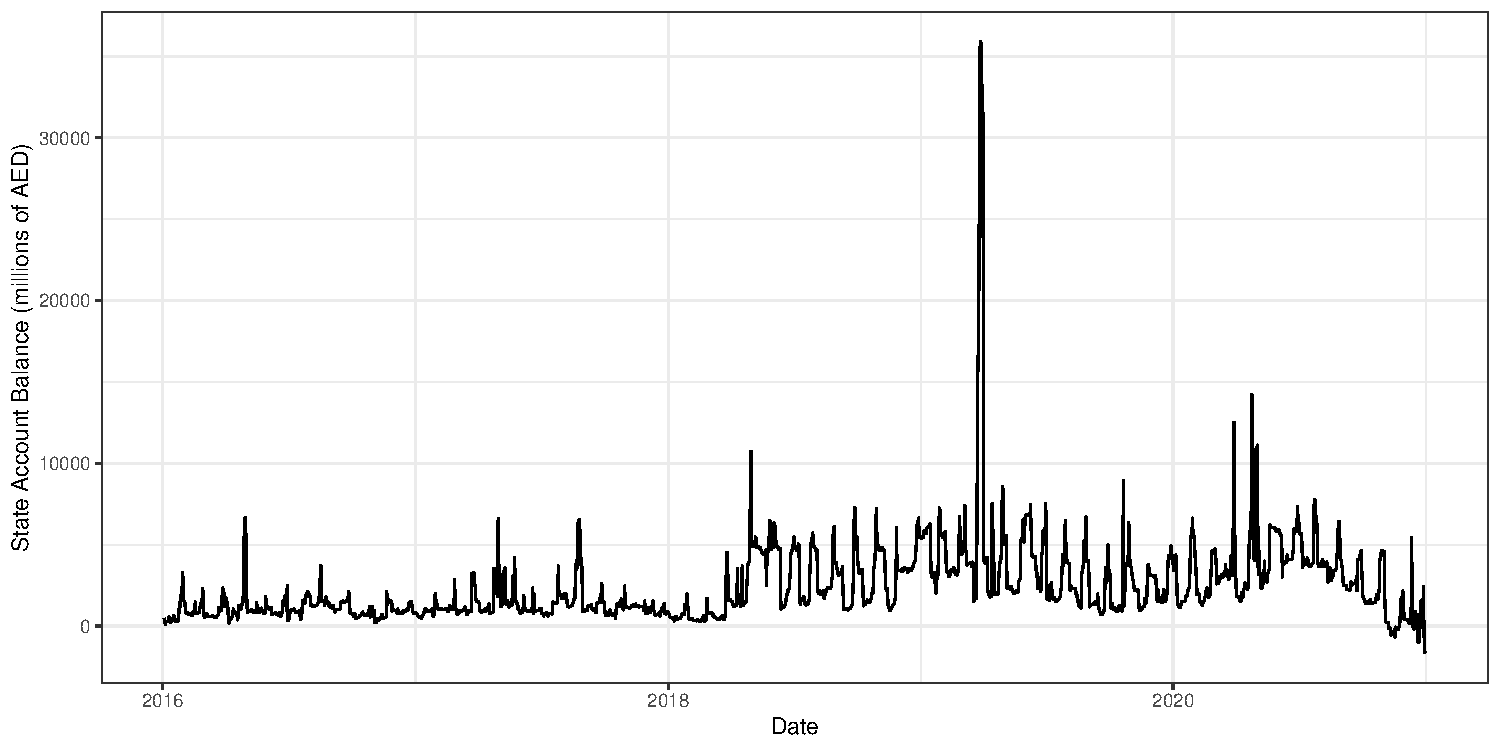
\includegraphics[scale=0.6]{sabplot}
    \caption{State Account Balance data for  the United Arab Emirates measured
in million of Dirhams.}
    \label{fig:sabdata}
\end{figure}

\subsection{Net Foreign Assets}

Net Foreign Assets (NFA)  is the total foreign assets held  by a central bank,
net of their foreign liabilities

\textit{\color{blue}  RF to  potentially expand  on NFA  data, how  collected,
measured etc.}

Compared  to other  autonomous factors,  NFA  are not  influenced by  calendar
effects and when  forecasting the mean, it is often  difficult to outperform a
na\"ive forecast  of last observed value  of NFA. However the  daily change in
NFA  do resemble  financial returns  in  that they  often exhibit  conditional
heteroskedasticity and volatility  clustering. This makes the  GARCH family of
models good  candidates for forecasting  the entire distribution of  NFA data,
which can be  a critical input into operational decisions  of Central Banks in
the money market.

Figure~\ref{fig:nfadata} shows both  the level (top panel)  and change (bottom
panel) in net foreign assets. The bottom panel in particular shows evidence of
conditional heteroskedasticity  motivating the use  of GARCH models  and their
extensions

\begin{figure}[!h] \centering 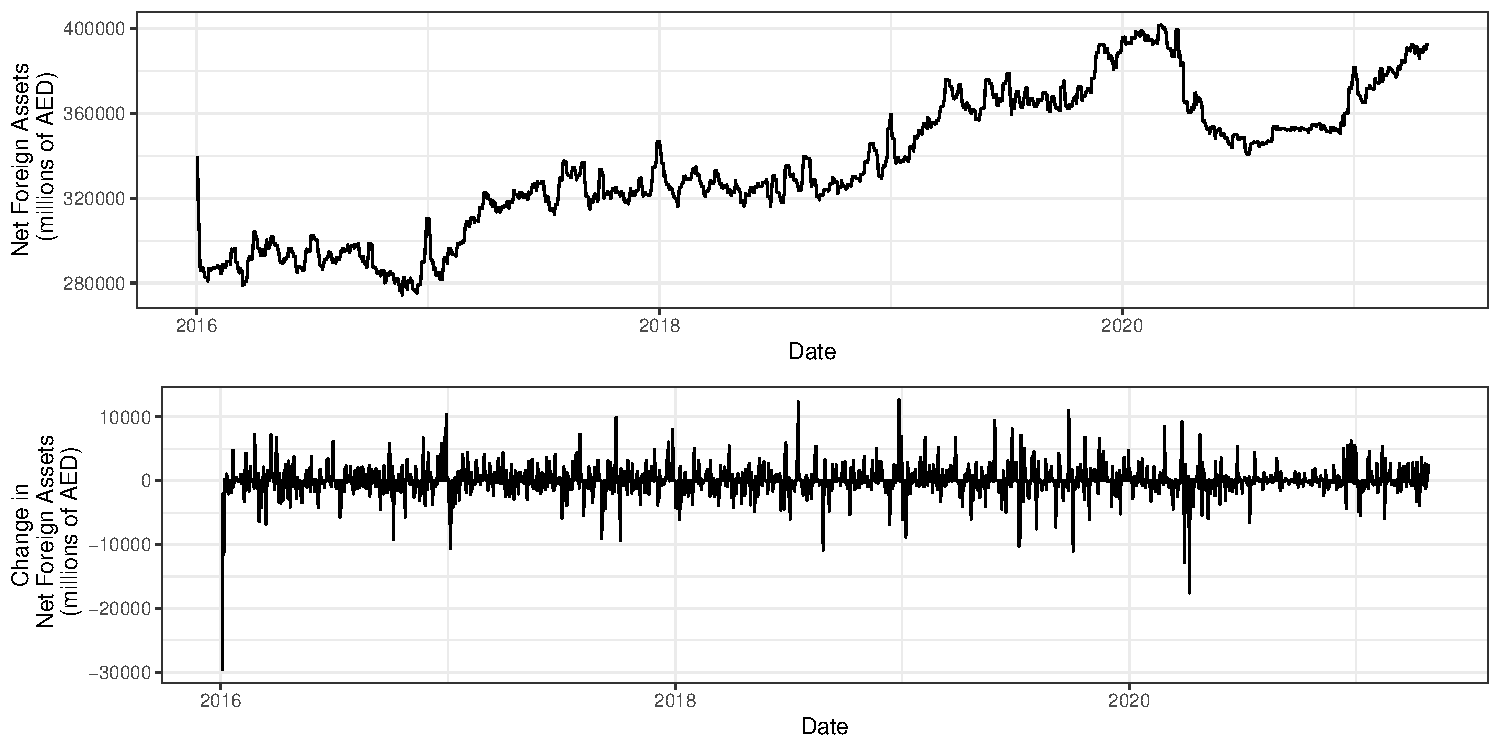
\includegraphics[scale=0.6]{nfaplot}
    \caption{Net Foreign Assets data for  the United Arab Emirates measured in
million of Dirhams. Top panel: level, bottom panel: change.}
    \label{fig:nfadata}
\end{figure}

\subsection{Aggregate}

The  aggregate (AGG)  for  the autonomous  factors (or  net  liquidity due  to
autonomous factors) is given by

\[ AGG=NFA-(CIC+SAB)
\]

This reflects the fact  that while NFA are clearly assets  on the central bank
balance sheet, CIC and SAB are  liabilities for a central bank. This aggregate
represents the net liquidity due  to autonomous factors.  While this aggregate
is composed  of all autonomous  factors, in general the  scale of NFA  is much
higher than  CIC and SAB. As  a result, the  high variability of NFA  tends to
dominate  this time  series.  Suitable  models for  forecasting the  aggregate
series are thus models for  conditional volatility.  However, information from
CIC  and SAB  can  be incorporated  into  the forecast  of  the aggregate  via
forecast   reconciliation   methodology,   discussed   in   more   detail   in
Section~\ref{sec:forereco}.

Figure~\ref{fig:aggdata} shows the net liquidity due to autonomous factors for
the UAE. The top panel shows the  level, the bottom panel shows the change. It
is clear that variability  of the NFA data dominates the  influence of CIC and
SAB.  While  the predictable  seasonal  patterns  of  CIC  and SAB  should  in
principle help with  forecasting the aggregate, it will be  difficult to model
these  effects  while  modelling  the  aggregate  series  alone.  Later,  this
motivates  forecast  reconciliation  approaches   where  separate  models  are
developed for each of the autonomous factors and the aggregate.

\begin{figure}[!h]
    \centering
    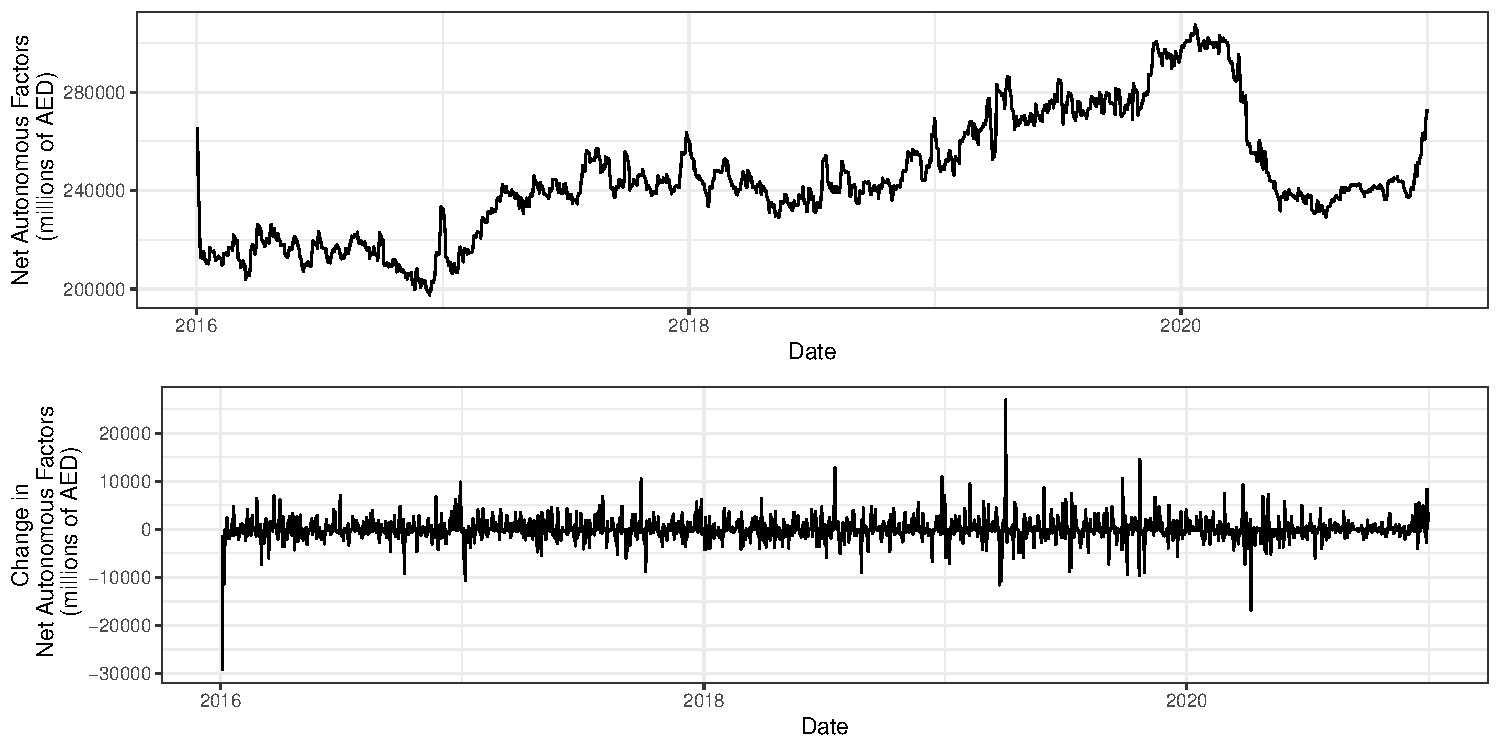
\includegraphics[scale=0.6]{aggplot}
    \caption{Net liquidity due to autonomous factors for the United Arab Emirates measured in million of Dirhams. Top panel: level, bottom panel: change.}
    \label{fig:aggdata}
\end{figure}

%%% Local Variables:
%%% mode: latex
%%% TeX-master: t
%%% End:
